\begin{center}
	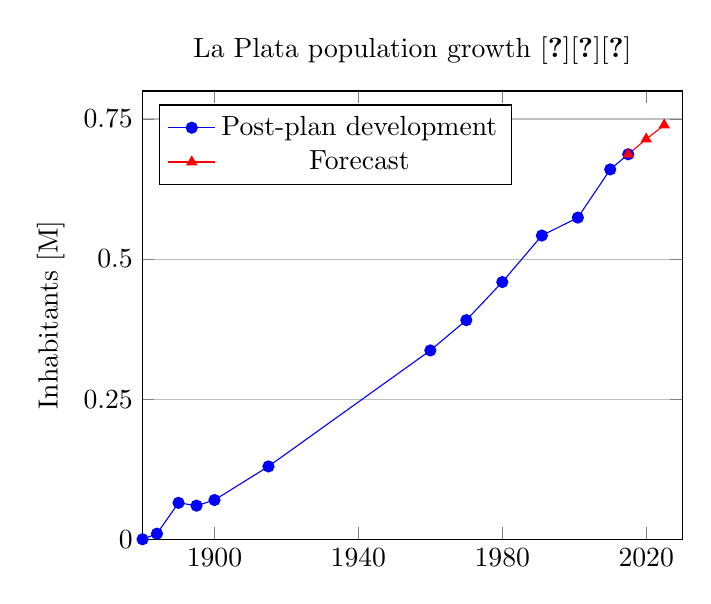
\begin{tikzpicture}[>=latex]
		\begin{axis}[
				title={La Plata population growth \cite{CityPopulation:LaPlata}\cite{Wikipeda:LaPlataHistory}\cite{ElDiaSa:LaPlata2025}},
				style={/pgf/number format/1000 sep=},
				ylabel={Inhabitants [M]},
				xmin=1880, xmax=2030,
				ymin=0, ymax=0.8,
				xtick={1900,1940,1980,2020},
				ytick={0,0.25,0.5,0.75},
				legend pos=north west,
				ymajorgrids=true
			]				
			\addplot[color=blue,mark=otimes*] coordinates {
				(1880,0)(1884,0.01)(1890,0.065)(1895,0.06)(1900,0.07)(1915,0.13)(1960,0.337)(1970,0.391)(1980,0.459)(1991,0.542)(2001,0.574)(2010,0.660)(2015,0.687)
			};
			\addplot[color=red,mark=triangle*] coordinates {
				(2015,0.687)(2020,0.714)(2025,0.739)
			};
			
			\legend{Post-plan development, Forecast}				
		\end{axis}
	\end{tikzpicture}	
\end{center}
